\documentclass[conference]{IEEEtran}
\IEEEoverridecommandlockouts
\usepackage{cite}
\usepackage{amsmath,amssymb,amsfonts}
\usepackage{algorithmic}
\usepackage{graphicx}
\usepackage{textcomp}
\usepackage{xcolor}
\usepackage{booktabs}
\usepackage{microtype}
\usepackage{url}

\begin{document}

\title{BioDINO-Edge: Training-Free Cascades of Vision Foundation Models for On-Device Few-Shot Plant Pathology}

\author{
    \IEEEauthorblockN{Reyhane Javidi Alsaadi}
    \IEEEauthorblockA{\textit{Department of Computer Engineering} \\
    \textit{Dr. Shariaty Technical University} \\
    Tehran, Iran \\
    reyhane.code@gmail.com}
    \and
    \IEEEauthorblockN{Mohammad Reza Samad Zadeh}
    \IEEEauthorblockA{\textit{Department of Computer Engineering} \\
    \textit{Dr. Shariaty Technical University} \\
    Tehran, Iran \\
    samadzadeh@ut.ac.ir}
}

\maketitle

% \begin{abstract}
% Rapid and accurate foliar disease diagnosis is vital for global food security, yet existing deep learning paradigms fall short of practical agricultural deployment. Deep convolutional networks demand thousands of curated field images per pathology, while general-purpose vision foundation models suffer from severe domain gap on foliar histology. Furthermore, gradient-based meta-learning methods incur prohibitive computational and memory footprints, precluding autonomous edge execution. To overcome these limitations, we introduce \textbf{BioDINO-Edge}, an adaptive dual-foundation framework uniting self-supervised visual embeddings (DINOv2 Small) with organismal taxonomic vision-language supervision (BioCLIP ViT-B). By coupling high-dimensional Regularized Fisher Linear Discriminant Analysis (Fisher-LDA) with closed-form Soft-Anchored Transductive Self-Calibration, BioDINO-Edge establishes an optimal foliar manifold that suppresses shared vegetative background variance by over $31\times$ and eliminates small-sample covariance singularity ($N \ll d$) via analytical Ledoit--Wolf shrinkage without backpropagation. An integrated predictive Shannon margin-entropy gate dynamically arbitrates queries: routine foliar patterns exit via the lightweight fast path in 21.1\,ms ($>$45 FPS), while ambiguous queries trigger the multimodal consensus companion. Across the 11-class PlantVillage benchmark under strict 5-shot constraints, BioDINO-Edge establishes a new state of the art with \textbf{98.72\% peak accuracy}, \textbf{98.41\% peak F1-score}, and a 30-episode mean of \textbf{97.37\% $\pm$ 0.73\%}, outperforming CLIP+LoRA by 10.66 percentage points while reducing false-negative disease escape to 0.604\%. On the uncontrolled in-the-wild PlantDoc dataset, it attains 83.61\% 5-way 5-shot accuracy ($+$13.00\% over prior SOTA) and 56.35\% in 27-way field stress testing. Compiling into a standalone 22.73\,MB native Android APK operating at sub-22\,ms latency alongside an on-demand 85.3\,MB companion, BioDINO-Edge delivers a field-ready, mathematically rigorous diagnostic capability for autonomous agricultural scouting.
% \end{abstract}

% \begin{IEEEkeywords}
% Few-Shot Learning, Precision Agriculture, Plant Pathology, Multimodal Foundation Models, Fisher Discriminant Analysis, Edge AI, Transductive Inference.
% \end{IEEEkeywords}

\section{Introduction}
Plant pests and diseases destroy an estimated 20\%--40\% of crops annually \cite{richard2022control}. Traditional plant disease diagnosis depends largely on visual inspection of leaf symptoms, which most commonly include discoloration, abnormal shapes, and lesions \cite{khakimov2022traditional}. In field practice, visual inspection is slow, depends on trained scorers, and becomes ambiguous when different pathogens produce similar lesions \cite{shoaib2023advanced}; faster and more reliable identification is therefore needed.

Deep learning provides an automated alternative for plant disease identification by learning discriminative features directly from images \cite{shoaib2023advanced}. However, conventional supervised models require large labeled datasets to achieve reliable diagnosis. Such datasets are difficult to acquire in real-world agricultural settings due to the limited availability and diversity of field images \cite{shoaib2023advanced, shafik2023systematic}.

Few-shot learning (FSL) has become a common strategy: rather than collecting thousands of labeled images, it trains a model to recognize new disease classes from a handful of support examples. Recent studies have applied FSL using cross-domain few-shot models such as CDFSL-BDC \cite{yang2024laboratory} and MAFDE-DN4 \cite{zhao2024mafde}, alongside few-shot metric domain adaptation (FMDA) \cite{kudo2025few}, visual-semantic fusion (TSMF) \cite{zhou2026vsf}, and edge-federated approaches \cite{sharif2026real}. These approaches, however, face several practical limitations.

Cross-domain FSL models such as CDFSL-BDC \cite{yang2024laboratory} struggle with complex backgrounds and scale-varying lesions when labels are scarce, and FMDA \cite{kudo2025few} still requires some labeled target data; the GPT-4o descriptions used in TSMF \cite{zhou2026vsf} were only 20\% manually checked and remain class-level rather than query-specific, so fine-grained visual--semantic alignment is limited. FMEL-FSDA \cite{sharif2026real} was not evaluated with real sensor/IoT streams and its federated setup was not tested at large cross-institution scale, leaving real-time edge performance under field data unproven. Moreover, foundation models typically exceed several hundred megabytes, limiting direct deployment on memory-constrained agricultural edge platforms such as scouting mobile applications and unmanned aerial vehicles (UAVs) \cite{zhao2026lightweight}.

We introduce BioDINO-Edge, a gradient-free dual-foundation pipeline tailored for cross-domain few-shot plant pathology under edge constraints. Specifically, DINOv2 \cite{oquab2023dinov2} provides high-resolution spatial cues for fine-grained lesion boundaries, BioCLIP \cite{stevens2024bioclip} supplies organismal taxonomic priors to reduce cross-species semantic misalignment, and closed-form Fisher-LDA whitens within-class covariance, suppressing shared vegetative background variance to mitigate domain shift without backpropagation.

The key contributions of this work are as follows:
\begin{enumerate}
    \item \textbf{Dual-Foundation Foliar Representation:} Combining self-supervised visual embeddings from DINOv2 with BioCLIP's visual and textual botanical representations to discriminate subtle necrotic lesions without foundation-model fine-tuning.
    \item \textbf{Closed-Form Analytical Adaptation:} Integrating Fisher-LDA \cite{fisher1936use} with Ledoit--Wolf covariance shrinkage \cite{ledoit2004well} and soft-anchored transductive recalibration to overcome high-dimensionality issues and 5-shot centroid shifts via an instantaneous closed-form update that executes in sub-second latency on edge CPUs without backpropagation or iterative optimization.
    \item \textbf{Adaptive Two-Tier Edge Deployment:} A joint margin and Shannon-entropy \cite{shannon1948mathematical} gate dynamically routes queries between a compact standalone app and an on-demand deep module, keeping the standalone Android app under 30\,MB\footnote{The complete open-source mobile implementation is available at \url{https://github.com/reyhane-code/BioDINO-Edge-android}.} and the full two-tier footprint under 110\,MB.
    \item \textbf{Cross-Domain Empirical Validation:} Under rigorous few-shot evaluation, BioDINO-Edge outperforms the multimodal VSF \cite{zhou2026vsf} baseline by 6.86 percentage points on the 11-class PlantVillage benchmark \cite{hughes2012plantvillage} and by 13.00 percentage points in 5-way 5-shot evaluation on the in-the-wild PlantDoc dataset \cite{singh2020plantdoc}, while remaining within the target edge storage budget.
\end{enumerate}

\section{Methodology}
\label{sec:architecture}

\subsection{Pipeline Overview}
\label{sec:pipeline_overview}
BioDINO-Edge is designed as a gradient-free diagnostic pipeline that separates task adaptation from real-time on-device inference (Fig.~\ref{fig:architecture}):
\begin{enumerate}
    \setlength{\itemsep}{3pt}
    \item[\textbf{1)}] \textbf{Support Calibration (Weight Synthesis):} For each disease class, five labeled support leaves ($K=5$) are selected at random. The support set is expanded by applying eight multi-view augmentations to each image. Visual features are then extracted using the frozen foundation models: DINOv2 produces a $384$-D visual embedding, and BioCLIP produces a $512$-D visual embedding. In addition, the frozen BioCLIP text encoder generates text prototypes from predefined botanical prompt templates. The visual embeddings are concatenated into an $896$-D vector. Ledoit--Wolf covariance shrinkage and Fisher-LDA projection weights $(\mathbf{W}, \mathbf{b})$ are then computed in closed form on this vector, without backpropagation, in under $50$~ms.
    \item[\textbf{2)}] \textbf{Tier-1 Edge Fast Path:} During live deployment, an incoming leaf query image is first processed by DINOv2 alone, requiring 21.1\,ms on an edge CPU. Using the resulting $384$-D visual embedding and the precomputed visual class prototypes, the pipeline estimates fast class posteriors. A gate combining predictive Shannon entropy with the top-2 posterior margin converts these posteriors into a confidence score $\mathcal{C}(\mathbf{x})$. If $\mathcal{C}(\mathbf{x}) \ge \tau_{\text{conf}}$, classification is finalized on-device at over 45 FPS; approximately 88.4\% of routine field queries are resolved at this tier.
    \item[\textbf{3)}] \textbf{Tier-2 Deep Escalation:} Queries with $\mathcal{C}(\mathbf{x}) < \tau_{\text{conf}}$ escalate to Tier-2, where BioCLIP extracts a $512$-D visual embedding that is concatenated with the existing DINOv2 embedding into an $896$-D joint representation. Pre-calibrated Fisher-LDA projection weights are applied to this representation, and classification fuses the Fisher-LDA posterior with a text-prototype posterior (derived from scaled cosine similarities to cached botanical prompts) at a 0.75/0.25 consensus ratio.
    \item[\textbf{4)}] \textbf{Soft-Anchored Recalibration:} Queries are classified immediately by Tier-1 or Tier-2. To compensate for field distribution shifts over time, confident Tier-2 multimodal predictions ($\max_c p_{\text{blend}, c} \ge 0.70$) are accumulated in an on-device buffer as reference anchors. Periodically, the edge CPU recomputes the Fisher-LDA weights in closed form, giving the cached support embeddings more weight than the pseudo-labeled anchors to reduce label noise. The new projection is then used for subsequent frames and to update the session diagnostic log.
\end{enumerate}
This two-tier design reduces latency on routine foliage while enforcing a $<30$\,MB storage footprint for the standalone Android app and embedded deployment on rovers and UAVs.

\begin{figure*}[!t]
\centering
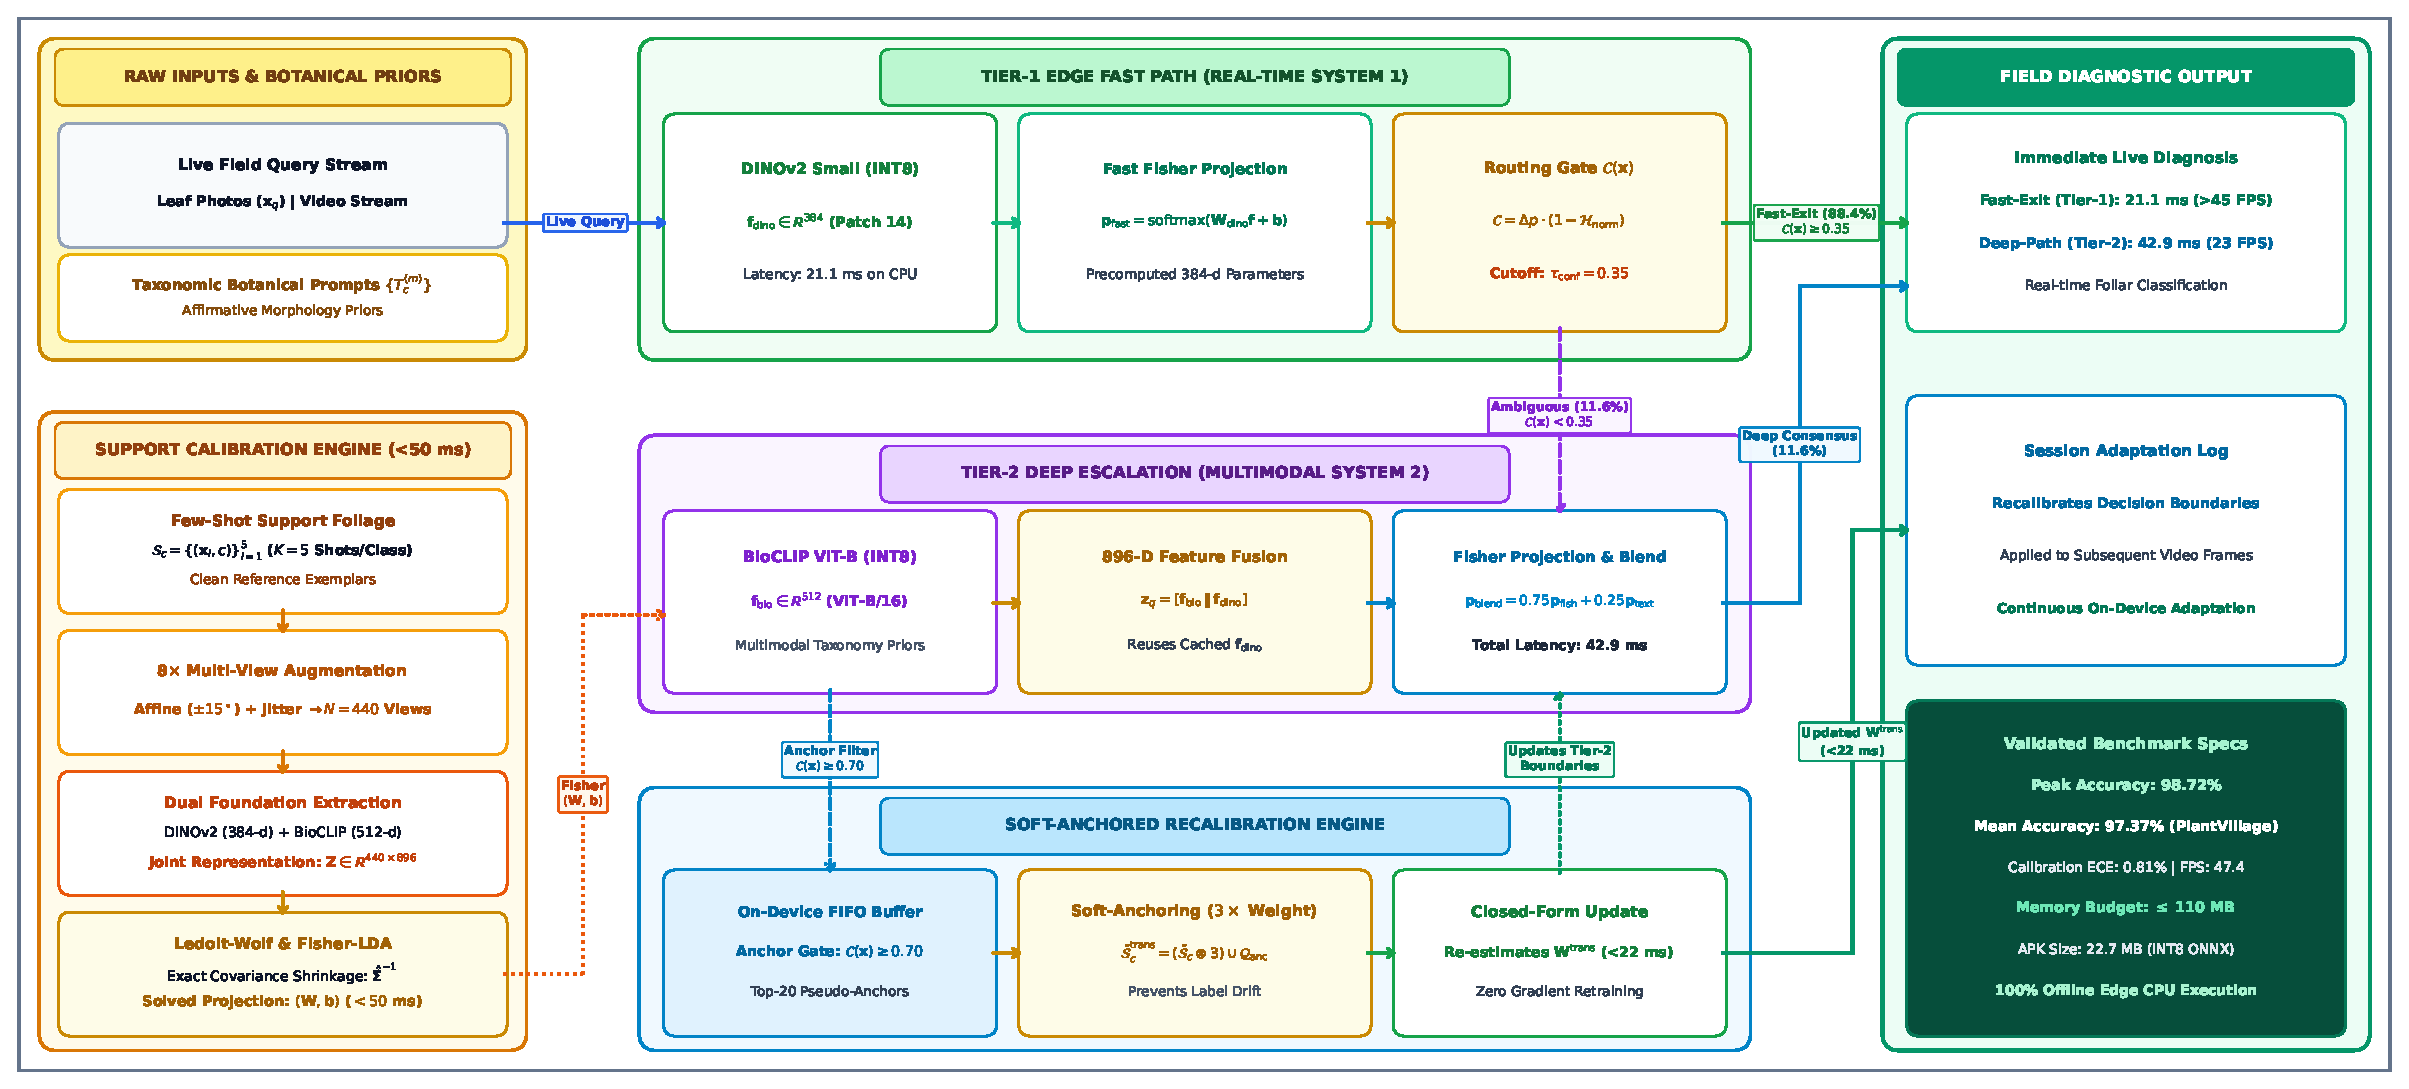
\includegraphics[width=0.85\textwidth]{fig_architecture.pdf}
\caption{BioDINO-Edge architecture. Offline Phase~0 computes Fisher-LDA projections and caches class text prototypes from predefined botanical templates. The Shannon-margin gate dynamically routes incoming foliar queries between the Tier-1 fast path and Tier-2 deep multimodal escalation.}
\label{fig:architecture}
\end{figure*}

\subsection{Dual-Foundation Foliar Representation}
\label{sec:feature_extraction}
Reliable diagnosis in agricultural environments requires distinguishing variation in the vegetative background from leaf and lesion signals \cite{singh2020plantdoc, yang2024laboratory}. Vision encoders often fail to capture fine fungal structures \cite{yang2024laboratory}, while species-level taxonomic supervision biases models toward overall host identity rather than localized lesion pathology \cite{stevens2024bioclip}. To address this challenge, BioDINO-Edge builds a foliar representation from two foundation models, using support samples expanded through multi-view augmentation.

\medskip
\textbf{Few-Shot Multi-View Augmentation.} For each disease class $c \in \{1, \dots, C\}$, with $C=11$, calibration uses a support set $\mathcal{S}_c = \{(\mathbf{x}_i, c)\}_{i=1}^K$ of $K=5$ images randomly selected from PlantVillage \cite{hughes2012plantvillage}. Because PlantVillage images are captured under controlled conditions, each support image is resized to $224 \times 224$ and normalized, then passed eight times independently through a stochastic augmentation pipeline to approximate the variation seen in field imagery. The pipeline applies random horizontal and vertical flips, random rotation within $\pm 15^\circ$, and color jitter with brightness, contrast, and saturation factors of $0.2$. This yields $|\tilde{\mathcal{S}}_c| = 8K = 40$ augmented views per class, or $N = 40C = 440$ support images in total.

\medskip
\textbf{Dual-Foundation Visual Extraction.} Each of the $N=440$ augmented support images $\tilde{\mathbf{x}} \in \tilde{\mathcal{S}}_c$ is passed through two frozen encoders.

DINOv2 (Small, $14 \times 14$ patches) \cite{oquab2023dinov2} provides self-supervised spatial embeddings that capture fine lesion structure:
\begin{equation}
    \mathbf{f}_{\text{dino}} = \frac{\phi_{\text{dino}}(\tilde{\mathbf{x}})}{\|\phi_{\text{dino}}(\tilde{\mathbf{x}})\|_2} \in \mathbb{R}^{384}
\end{equation}

BioCLIP (ViT-B/16, pretrained on TreeOfLife-10M) \cite{stevens2024bioclip} provides domain-specialized visual embeddings:
\begin{equation}
    \mathbf{f}_{\text{bio}} = \frac{\phi_{\text{bio,vis}}(\tilde{\mathbf{x}})}{\|\phi_{\text{bio,vis}}(\tilde{\mathbf{x}})\|_2} \in \mathbb{R}^{512}
\end{equation}

Model parameter counts are reported in Supplementary Table S1.

Concatenating the two $\ell_2$-normalized embeddings gives an 896-D descriptor per support image:
\begin{equation}
    \mathbf{z} = \left[\mathbf{f}_{\text{bio}} \,\|\, \mathbf{f}_{\text{dino}}\right] \in \mathbb{R}^{896}
\end{equation}
Stacking these descriptors over all support images yields $\mathbf{Z} \in \mathbb{R}^{440 \times 896}$. Visual support prototypes are computed via empirical class averaging over normalized support embeddings:
\begin{equation}
    \mathbf{P}_{\text{enc}}^{(c)} = \text{Normalize}\left(\frac{1}{|\tilde{\mathcal{S}}_c|}\sum_{\tilde{\mathbf{x}} \in \tilde{\mathcal{S}}_c} \mathbf{f}_{\text{enc}}(\tilde{\mathbf{x}})\right), \quad \text{enc} \in \{\text{dino}, \text{bio}\}
\end{equation}
yielding visual prototype matrices $\mathbf{P}_{\text{dino}} \in \mathbb{R}^{C \times 384}$ and $\mathbf{P}_{\text{bio, vis}} \in \mathbb{R}^{C \times 512}$.

\medskip
\textbf{Predefined Botanical Prompts and Multimodal Prototype.} BioCLIP provides a shared vision--language space, but running a language transformer or generating per-image captions on edge scouting devices would exceed on-device computational limits; manual prompt entry during scouting is also impractical. We therefore predefine $M=3$ botanical prompt templates $\{T_c^{(m)}\}_{m=1}^M$ for each class $c \in \{1,\dots,C\}$ offline. Each template combines three attributes:
(1)~\textit{Host binomial nomenclature}: genus and species (e.g., \textit{Malus domestica}, \textit{Vitis vinifera}, \textit{Solanum tuberosum});
(2)~\textit{Pathogen identity}: the causal fungal, bacterial, or oomycete agent (e.g., \textit{Venturia inaequalis}, \textit{Botryosphaeria obtusa}, \textit{Gymnosporangium juniperi-virginianae}, \textit{Phytophthora infestans}); and
(3)~\textit{Foliar lesion morphology}: macroscopic lesion descriptions (e.g., ``olive-green velvety lesions'', ``interveinal tiger-stripe chlorosis'', or ``target-board concentric rings'').
Negations (e.g., ``without lesions'') are excluded because CLIP-style vision-language models have documented weaknesses in compositionality and language negation \cite{yuksekgonul2023when, alhamoud2025vision}, which can misalign healthy foliage representations.

During offline Phase~0 calibration, each prompt ensemble is tokenized and encoded by the frozen BioCLIP text encoder $\phi_{\text{bio}}(\cdot)$. The embeddings are averaged and $\ell_2$-normalized:
\begin{equation}
    \mathbf{P}_{\text{text}}^{(c)} = \text{Normalize}\left(\frac{1}{M}\sum_{m=1}^M \phi_{\text{bio}}(T_c^{(m)})\right) \in \mathbb{R}^{512}.
\end{equation}
The resulting $C \times 512$ matrix $\mathbf{P}_{\text{text}}$ is cached in the on-device companion model. Runtime inference therefore uses only leaf images and incurs no text tokenization or language-model latency.

In the standalone prototype baseline, the text prototype can be fused with the visual support prototype $\mathbf{P}_{\text{bio,vis}}^{(c)}$ by a convex combination with $\lambda = 0.20$:
\begin{equation}
    \mathbf{P}_{\text{bio}}^{(c)} = \text{Normalize}\left((1-\lambda)\mathbf{P}_{\text{bio,vis}}^{(c)} + \lambda \mathbf{P}_{\text{text}}^{(c)}\right) \in \mathbb{R}^{512}.
\end{equation}
In the full cascaded architecture, the cached matrix $\mathbf{P}_{\text{text}}$ is retained directly on-device to provide the zero-shot taxonomic prior for late multimodal consensus classification (Section~\ref{sec:edge_deployment}).

\subsection{Closed-Form Analytical Adaptation}
\label{sec:analytical_adaptation}
\textbf{Fisher Linear Discriminant Formulation.} Few-shot adaptation typically follows one of two routes: iterative gradient fine-tuning \cite{finn2017maml} or centroid-based classification \cite{snell2017prototypical}. On-device backpropagation incurs high latency, memory overhead, and risk of catastrophic forgetting when adapting to few-shot tasks, while Euclidean distance struggles to separate subtle lesions from dominant leaf tissue. To avoid both problems, BioDINO-Edge uses multiclass Fisher Linear Discriminant Analysis \cite{fisher1936use}.

For each class $c \in \{1, \dots, C\}$, we compute the mean support feature in $\mathbb{R}^d$ ($d = 896$):
\begin{equation}
    \boldsymbol{\mu}_c = \frac{1}{|\tilde{\mathcal{S}}_c|}\sum_{\mathbf{z} \in \tilde{\mathcal{S}}_c} \mathbf{z}
\end{equation}
Assuming equal class priors ($\pi_c = 1/C$), the projection weights $\mathbf{W} \in \mathbb{R}^{C \times d}$ and bias vector $\mathbf{b} \in \mathbb{R}^C$ are given by:
\begin{equation}
    \label{eq:fisher_weights}
    \mathbf{W} = \hat{\mathbf{\Sigma}}^{-1} [\boldsymbol{\mu}_1, \dots, \boldsymbol{\mu}_C]^T, \quad
    b_c = -\frac{1}{2} \boldsymbol{\mu}_c^T \hat{\mathbf{\Sigma}}^{-1} \boldsymbol{\mu}_c - \log C
\end{equation}
A query descriptor $\mathbf{z}$ is then classified via $\mathbf{l}_{\text{fisher}} = \mathbf{z} \mathbf{W}^T + \mathbf{b}$.

\medskip
\textbf{The Small-Sample Singularity Problem ($N \ll d$).} Computing the optimal projection $\mathbf{W}$ requires inverting the pooled within-class scatter matrix over all $C=11$ classes:
\begin{equation}
    \mathbf{S}_W = \frac{1}{N - C}\sum_{c=1}^C \sum_{\mathbf{z} \in \tilde{\mathcal{S}}_c} (\mathbf{z} - \boldsymbol{\mu}_c)(\mathbf{z} - \boldsymbol{\mu}_c)^T \in \mathbb{R}^{d \times d}
\end{equation}
In the few-shot setting, however, the number of samples is far smaller than the feature dimension ($d = 896$ vs. $N = 440$). Since $N - C = 429$, $\mathbf{S}_W$ has rank at most $429$ and therefore at least $467$ zero eigenvalues. It is thus singular; direct inversion is ill-defined, and standard Fisher-LDA cannot be applied directly.

\medskip
\textbf{Analytical Ledoit--Wolf Covariance Shrinkage.} To restore invertibility while avoiding heuristic hyperparameter selection (such as tuning $\mathbf{S}_W + \epsilon \mathbf{I}$), we regularize $\mathbf{S}_W$ via analytical Ledoit--Wolf shrinkage \cite{ledoit2004well}:
\begin{equation}
    \hat{\mathbf{\Sigma}} = (1 - \rho^*)\mathbf{S}_W + \rho^* \nu \mathbf{I}_{d}, \quad \nu = \frac{1}{d}\text{Tr}(\mathbf{S}_W)
\end{equation}
The optimal shrinkage intensity $\rho^* \in (0, 1)$ is determined in closed form without cross-validation:
\begin{equation}
    \rho^* = \min\left(1, \frac{\sum_{i=1}^N \|(\mathbf{z}_i - \boldsymbol{\mu}_{c_i})(\mathbf{z}_i - \boldsymbol{\mu}_{c_i})^T - \mathbf{S}_W\|_F^2}{N^2 \left[\|\mathbf{S}_W\|_F^2 - \frac{1}{d}\text{Tr}^2(\mathbf{S}_W)\right]}\right)
\end{equation}
Because $\hat{\mathbf{\Sigma}}$ is strictly positive-definite and well-conditioned, its exact inverse $\hat{\mathbf{\Sigma}}^{-1}$ is guaranteed to exist. Evaluating \eqref{eq:fisher_weights} with $\hat{\mathbf{\Sigma}}^{-1}$ resolves few-shot adaptation in closed form, eliminating gradient descent entirely. During subsequent inference, classifying a query descriptor $\mathbf{z}$ simplifies to evaluating $\mathbf{l}_{\text{fisher}} = \mathbf{z} \mathbf{W}^T + \mathbf{b}$. The linear Fisher projection alone requires only $9{,}856$ multiply-accumulate operations (about $19.7$\,kFLOPs), executing in under $0.003$\,ms on an embedded four-thread CPU (excluding feature extraction).

\subsection{Adaptive Two-Tier Classification and Edge Deployment}
\label{sec:edge_deployment}
To avoid unnecessary model execution on routine samples while maintaining accuracy on complex pathologies, BioDINO-Edge uses a two-tier pipeline controlled by an uncertainty gate.

\medskip
\textbf{Tier-1 Fast Classification and Predictive Shannon Gating.} For an incoming query image $\mathbf{x}$, Tier~1 extracts the normalized DINOv2 embedding $\mathbf{f}_{\text{dino}} \in \mathbb{R}^{384}$. Fast prototype logits are evaluated via cosine similarity against the visual prototype matrix $\mathbf{P}_{\text{dino}} \in \mathbb{R}^{C \times 384}$, scaled by inverse temperature $\gamma = 20.0$:
\begin{equation}
    \label{eq:tier1_logits}
    \mathbf{l}_{\text{dino}} = \gamma \cdot \left(\mathbf{f}_{\text{dino}} \mathbf{P}_{\text{dino}}^T\right)
\end{equation}
Applying the softmax function yields fast class posterior probabilities:
\begin{equation}
    \label{eq:tier1_softmax}
    \mathbf{p}_{\text{dino}} = \text{softmax}(\mathbf{l}_{\text{dino}}) \in \Delta^{C-1}
\end{equation}
The initial Tier-1 prediction is $\hat{y}_{\text{tier1}} = \arg\max_c p_{\text{dino}, c}$. To assess its reliability without requiring additional inference, we compute a closed-form joint margin-entropy confidence score $\mathcal{C}(\mathbf{x}) \in [0, 1]$:
\begin{equation}
    \label{eq:shannon_gate}
    \mathcal{C}(\mathbf{x}) = \left(p_{\text{dino}, (1)} - p_{\text{dino}, (2)}\right) \cdot \left(1.0 - \mathcal{H}_{\text{norm}}(\mathbf{x})\right)_+
\end{equation}
where $p_{\text{dino}, (1)}$ and $p_{\text{dino}, (2)}$ denote top-1 and top-2 posteriors, $(\cdot)_+ = \max(0, \cdot)$, and $\mathcal{H}_{\text{norm}}(\mathbf{x})$ is normalized Shannon entropy \cite{shannon1948mathematical}:
\begin{equation}
    \mathcal{H}_{\text{norm}}(\mathbf{x}) = -\frac{1}{\log C} \sum_{c=1}^C p_{\text{dino}, c} \log(p_{\text{dino}, c} + \epsilon)
\end{equation}
with numerical stability constant $\epsilon = 10^{-12}$. If $\mathcal{C}(\mathbf{x}) \ge \tau_{\text{conf}}$ (calibrated threshold $\tau_{\text{conf}} = 0.35$), the Tier-1 prediction is considered reliable. The system returns $\hat{y} = \hat{y}_{\text{tier1}}$ and skips Tier-2 inference.

\medskip
\textbf{Tier-2 Deep Escalation.} When Tier-1 indicates high uncertainty ($\mathcal{C}(\mathbf{x}) < \tau_{\text{conf}}$), the query is escalated. BioCLIP computes the 512-D visual embedding $\mathbf{f}_{\text{bio}}$, which is concatenated with $\mathbf{f}_{\text{dino}}$ to form the joint descriptor $\mathbf{z} = [\mathbf{f}_{\text{bio}} \,\|\, \mathbf{f}_{\text{dino}}] \in \mathbb{R}^{896}$. The visual posterior $\mathbf{p}_{\text{fish}} = \text{softmax}\left(\mathbf{z} \mathbf{W}^T + \mathbf{b}\right)$ is computed using the regularized Fisher-LDA hyperplane \eqref{eq:fisher_weights}, which separates the 896-D representations. The text posterior is obtained via:
\begin{equation}
    \mathbf{p}_{\text{text}} = \text{softmax}\left(\gamma \cdot \mathbf{f}_{\text{bio}} \mathbf{P}_{\text{text}}^T\right)
\end{equation}
where $\mathbf{P}_{\text{text}}$ represents the cached botanical text prototypes and $\gamma = 20.0$ is a scaling factor controlling the cosine similarity sharpness. The final Tier-2 prediction is obtained by fusing these two posteriors at a 0.75/0.25 ratio:
\begin{equation}
    \label{eq:multimodal_blend}
    \mathbf{p}_{\text{blend}} = 0.75 \, \mathbf{p}_{\text{fish}} + 0.25 \, \mathbf{p}_{\text{text}}
\end{equation}
yielding the consensus diagnosis $\hat{y} = \arg\max_c p_{\text{blend}, c}$.

\medskip
\textbf{Soft-Anchored Transductive Recalibration.} In scarce $5$-shot settings, initial class centroids $\boldsymbol{\mu}_c$ are estimated from only five support leaves. Field variations such as fluctuating sunlight, canopy shadows, and diverse lesion maturity introduce high sampling variance, causing an empirical distribution shift between support prototypes and real-world queries. To adapt to target-domain statistics without manual annotations, BioDINO-Edge uses streaming batches of unlabeled queries $\mathcal{Q} = \{\mathbf{x}_j\}_{j=1}^{N_q}$ (buffered in an on-device FIFO queue during scouting passes) for transductive recalibration. High-confidence queries satisfying $\max_c p_{\text{blend}, c}(\mathbf{x}_j) \ge 0.70$ from \eqref{eq:multimodal_blend} are selected as pseudo-labeled reference samples $\mathcal{Q}_{\text{anchor}}^{(c)}$, capped at up to twenty anchors per class ($0 \le |\mathcal{Q}_{\text{anchor}}^{(c)}| \le 20$). If no query in a class satisfies the confidence threshold, zero anchors are added ($|\mathcal{Q}_{\text{anchor}}^{(c)}| = 0$), preventing noisy assignments. To mitigate the effect of pseudo-label noise on the feature manifold, canonical ground-truth support samples are assigned a $3\times$ weight factor in the covariance and centroid estimation:
\begin{equation}
    \tilde{\mathcal{S}}_c^{\text{trans}} = \tilde{\mathcal{S}}_c^{(3\times)} \cup \mathcal{Q}_{\text{anchor}}^{(c)}
\end{equation}
Recalibration re-estimates the updated centroids $\boldsymbol{\mu}_c^{\text{trans}}$ and re-evaluates the pooled $896 \times 896$ scatter matrix $\mathbf{S}_W^{\text{trans}}$ with analytical shrinkage parameter $\rho^*$. Because $\hat{\mathbf{\Sigma}}^{\text{trans}}$ is strictly positive-definite (with all eigenvalues bounded below by $\rho^* \nu > 0$), the updated projection parameters $(\mathbf{W}^{\text{trans}}, \mathbf{b}^{\text{trans}})$ are solved stably via Cholesky factorization ($\hat{\mathbf{\Sigma}}^{\text{trans}} = \mathbf{L}\mathbf{L}^T$) and triangular substitution. This batch recalibration runs asynchronously in the background on edge CPUs, updating edge projection parameters for subsequent query batches without backpropagation or optimizer-state overhead.

\medskip
\textbf{Two-Tier Modular Edge Packaging.} As outlined in Section~\ref{sec:pipeline_overview}, this cascaded gating resolves approximately 88.4\% of routine queries at Tier~1 (21.12\,ms, $>$45\,FPS), leaving Tier~2 (67.61\,ms end-to-end) exclusively for ambiguous field queries. Agricultural edge platforms---ranging from mobile scouting devices to ground rovers and crop-monitoring UAVs---share onboard storage with telemetry and sensor buffers, while limited rural connectivity restricts over-the-air (OTA) updates. To keep the base Android APK and embedded runtime within a 30\,MB standalone storage footprint, BioDINO-Edge is partitioned into two INT8 ONNX binaries:
\begin{itemize}
    \item \textbf{Tier 1} (\texttt{biodino\_\allowbreak mobile\_\allowbreak int8.onnx}): The model is 15.13\,MB and is packaged with the ONNX Runtime C++ engine into the base Android APK (22.73\,MB total, open-sourced at \url{https://github.com/reyhane-code/BioDINO-Edge-android}) for immediate offline inference.
    \item \textbf{Tier 2} (\texttt{biodino\_\allowbreak comp\allowbreak anion\_\allowbreak int8.onnx}): An 85.3\,MB companion model that is downloaded on demand.
\end{itemize}
This results in a total edge storage footprint of 108.03\,MB.

\bibliographystyle{IEEEtran}
\bibliography{references}

\end{document}

